\documentclass[12pt,a4paper]{article}
\usepackage[a4paper,top=12mm,bottom=12mm,left=15mm,right=15mm]{geometry}
\usepackage[T1]{fontenc}
\usepackage{amsmath}
\usepackage{amssymb}
% A sans serif font with a single-storey a, as children write it. It is
% used for the mathematics as well as the text.
\usepackage{tgadventor}
\renewcommand*{\familydefault}{\sfdefault}
\usepackage[italic]{mathastext}
\usepackage{enumitem}
\usepackage{xcolor}
\usepackage{tikz}
\usepackage[most]{tcolorbox}

% ================================================================
% Constructions and loci.
%
% Pupils already know how to construct the perpendicular bisector of
% a line segment, the perpendicular to a line at a point on the line,
% and the perpendicular from a point to a line, so there are no
% worked examples.
%
% Pages 1 to 3 are assorted construction questions. Pages 1 and 2
% have each construction on its own, with the lines at different
% angles, and page 3 uses the constructions to find the height of a
% triangle, to draw a square and to find the centre of a circle.
%
% Pages 4 to 8 introduce loci. The first two loci questions mark some
% of the points that follow a rule before the locus is drawn, so that
% pupils see why the locus is a circle, and why the perpendicular
% bisector is the locus of the points equidistant from two points.
% The next question puts these two loci together to make a region.
% Then come the shortest distance from a point to a line (the
% perpendicular from the point), the points a fixed distance from a
% line (two parallel lines, drawn with perpendiculars at two points),
% and the points a fixed distance from a line segment. The scaffolding
% fades from there: a region with three rules and no steps, a mast
% the same distance from three villages, and a treasure map that ends
% with clues of the pupils' own.
%
% The sheet is eight sides of A4, so it can be printed as a booklet
% on two sheets of A3. The \newpage commands are placed so that no
% question is split across a page.
%
% Pupils construct on the sheet, so every diagram is drawn to scale
% (1 unit in TikZ is 1 cm). The sheet has to be printed at actual
% size: "fit to page" shrinks the diagrams and changes the answers
% that are measured. The answers are in a comment beside each
% question.
% ================================================================

\pagestyle{empty}
\setlength{\parindent}{0pt}
\setlength{\parskip}{0pt}
% Ragged right, so that the spaces between words are all the same, and
% no words broken across lines. A minipage sets the text justified
% again, so each side-by-side column starts with \raggedright as well.
\AtBeginDocument{\raggedright}
\hyphenpenalty=10000
\exhyphenpenalty=10000
\setlist[enumerate]{label=(\alph*), leftmargin=*, itemsep=7pt,
  topsep=4pt, parsep=0pt}
\setlist[itemize]{leftmargin=*, itemsep=3pt, topsep=4pt, parsep=0pt}

% The idea the loci questions are built on, boxed and only faintly
% tinted, so the sheet is cheap to print.
\newtcolorbox{keyidea}{colback=orange!3,colframe=orange!35,boxrule=0.6pt,
  left=6pt,right=6pt,top=5pt,bottom=5pt}

\newcommand{\sheettitle}[1]{\begin{center}{\LARGE\bfseries #1}\end{center}
  \vspace{-6pt}}
% An instruction for the questions after it.
\newcommand{\instruction}[1]{\par{\large\bfseries #1}\par\vspace{6pt}}

% The questions are numbered with a counter, so that they can be moved.
\newcounter{qn}
\newcommand{\q}{\refstepcounter{qn}\textbf{Q\theqn.}\ }

% An answer line at the right-hand end of a question, with the units
% after it: \answer{2cm}{cm}. It goes on the last line of the question
% if there is room, and on a line of its own if not. (This is the
% \signed macro from The TeXbook, with \hfill in place of \hfil so
% that it still reaches the right margin when the text is ragged
% right.)
\newcommand{\gapstrut}{\rule[-1.5mm]{0pt}{7.5mm}}
\newcommand{\answer}[2]{{\unskip\nobreak\hfill\penalty50
  \hskip2em\hbox{}\nobreak\hfill\gapstrut\underline{\hspace{#1}}\,#2%
  \parfillskip=0pt \finalhyphendemerits=0 \par}}
% A gap in a sentence.
\newcommand{\gap}[1]{\gapstrut\underline{\hspace{#1}}}
% A full-width line to write an explanation on.
\newcommand{\wline}{\par\vspace{16pt}\noindent\rule{\linewidth}{0.4pt}}

% ----------------------------------------------------------------
% Diagrams. Every one is drawn at actual size. The bounding box of
% each picture is set by hand, to leave room around the lines for the
% construction arcs.
\tikzset{
  given/.style={line width=0.7pt},
  extension/.style={line width=0.7pt, dash pattern=on 3pt off 2.5pt},
  lab/.style={inner sep=3pt},
  note/.style={font=\small, inner sep=2pt},
}
% A point labelled with a letter: \pt{(x,y)}{label position}{letter}.
\newcommand{\pt}[3]{\fill #1 circle (1.5pt); \node[lab,#2] at #1 {$#3$};}
% A point on a map, labelled with what it is and its letter:
% \place{(x,y)}{label position}{pond $P$}.
\newcommand{\place}[3]{\fill #1 circle (1.5pt); \node[lab,#2] at #1 {#3};}
% A diagram under a question, centred, without the space that the
% center environment puts round it.
\newenvironment{diagram}{\par\vspace{8pt}\centering}{\par}

\begin{document}

% ================================================================
% PAGE 1: one of each construction, on horizontal lines
% ================================================================

\sheettitle{Constructions and Loci}

\instruction{Use a ruler and a pair of compasses.\\
Do not rub out your construction arcs.}

% Q1: the perpendicular bisector is the vertical line through the
% midpoint of AB, 4 cm from A.
\q Construct the perpendicular bisector of the line segment $AB$.

\begin{diagram}
\begin{tikzpicture}
  \useasboundingbox (-1,-3.4) rectangle (9,3.4);
  \draw[given] (0,0) -- (8,0);
  \pt{(0,0)}{left}{A}
  \pt{(8,0)}{right}{B}
\end{tikzpicture}
\end{diagram}

\vfill

% Q2: the perpendicular from P meets the line 8 cm from its left-hand
% end. The distance from P to the line is 3 cm.
\q Construct the perpendicular from the point $P$ to the line.
Then measure the distance from $P$ to the line. \answer{2cm}{cm}

\begin{diagram}
\begin{tikzpicture}
  \useasboundingbox (-0.3,-3.3) rectangle (13,3.5);
  \draw[given] (0,0) -- (13,0);
  \pt{(8,3)}{above}{P}
\end{tikzpicture}
\end{diagram}

\vfill

% Q3: the perpendicular at Q is the vertical line through Q.
\q Construct the perpendicular to the line at the point $Q$.

\begin{diagram}
\begin{tikzpicture}
  \useasboundingbox (-0.3,-0.8) rectangle (13,4.4);
  \draw[given] (0,0) -- (13,0);
  \pt{(4.5,0)}{below}{Q}
\end{tikzpicture}
\end{diagram}

\vfill
\newpage

% ================================================================
% PAGE 2: the same constructions, with the lines at other angles
% ================================================================

% Q4: the line is at 20 degrees to the horizontal, and R is 3 cm
% from it. The distance from R to the line is 3 cm.
\q Construct the perpendicular from the point $R$ to the line.
Then measure the distance from $R$ to the line. \answer{2cm}{cm}

\begin{diagram}
\begin{tikzpicture}
  \useasboundingbox (-0.3,-1.3) rectangle (12.2,5);
  \begin{scope}[rotate=20]
    \draw[given] (0,0) -- (12.5,0);
    \pt{(6.5,-3)}{below}{R}
  \end{scope}
\end{tikzpicture}
\end{diagram}

\vfill

% Q5: CD is 7 cm long, at 40 degrees to the horizontal, so CM is
% 3.5 cm.
% Q6: the perpendicular at S is the horizontal line through S.
\noindent
\begin{minipage}[t]{0.48\linewidth}\raggedright
\q Construct the perpendicular bisector of the line segment $CD$.
Mark the midpoint $M$ of $CD$, and measure the length of $CM$.
\answer{2cm}{cm}

\vspace{6pt}
\centering
\begin{tikzpicture}
  \useasboundingbox (-4,-3.3) rectangle (4,3.3);
  \begin{scope}[rotate=40]
    \draw[given] (-3.5,0) -- (3.5,0);
    \pt{(-3.5,0)}{below left}{C}
    \pt{(3.5,0)}{above right}{D}
  \end{scope}
\end{tikzpicture}
\end{minipage}\hfill
\begin{minipage}[t]{0.48\linewidth}\raggedright
\q Construct the perpendicular to the line at the point $S$.

\vspace{6pt}
\centering
\begin{tikzpicture}
  \useasboundingbox (-4,-3.3) rectangle (4,3.3);
  \draw[given] (-1.2,-3.3) -- (-1.2,3.3);
  \pt{(-1.2,-0.6)}{left}{S}
\end{tikzpicture}
\end{minipage}

\vfill

% Q7: (c) both perpendiculars are at right angles to the same line,
% so they are parallel.
\q
\begin{minipage}[t]{0.92\linewidth}\raggedright
\begin{enumerate}[topsep=0pt]
  \item Construct the perpendicular from the point $G$ to the line.
  \item Construct the perpendicular to the line at the point $H$.
  \item What do you notice about your two perpendiculars? \answer{5cm}{}
\end{enumerate}
\end{minipage}

\begin{diagram}
\begin{tikzpicture}
  \useasboundingbox (-0.3,-2.9) rectangle (13.5,3.6);
  \draw[given] (0,0) -- (13.5,0);
  \pt{(3,2.5)}{above}{G}
  \pt{(9.5,0)}{below}{H}
\end{tikzpicture}
\end{diagram}

\vfill
\newpage

% ================================================================
% PAGE 3: using the constructions
% ================================================================

% Q8: the perpendicular from C meets AB 2 cm from A. The height is
% 4 cm, and the area is 1/2 x 7 x 4 = 14 cm^2.
% Q9: the perpendiculars at E and F, with G and H 4 cm up them, give
% the square EFGH. The diagonal EG is 5.7 cm (4 x sqrt 2 = 5.66).
\noindent
\begin{minipage}[t]{0.48\linewidth}\raggedright
\q The diagram shows the triangle $ABC$.
\begin{enumerate}
  \item Construct the perpendicular from $C$ to the line segment $AB$.
  \item The perpendicular from $C$ to $AB$ is the height of the triangle.
    Measure the height. \answer{1.6cm}{cm}
  \item The base $AB$ is 7\,cm long. Work out the area of the
    triangle $ABC$. \answer{1.6cm}{cm$^2$}
\end{enumerate}

\vspace{8pt}
\centering
\begin{tikzpicture}
  \useasboundingbox (-0.8,-3.2) rectangle (7.8,4.6);
  \draw[given, line join=round] (0,0) -- (7,0) -- (2,4) -- cycle;
  \pt{(0,0)}{below left}{A}
  \pt{(7,0)}{below right}{B}
  \pt{(2,4)}{above}{C}
\end{tikzpicture}
\end{minipage}\hfill
\begin{minipage}[t]{0.48\linewidth}\raggedright
\q The points $E$ and $F$ are on the line, 4\,cm apart.
\begin{enumerate}
  \item Construct the perpendicular to the line at $E$, and the
    perpendicular to the line at $F$.
  \item Use your compasses to mark the point $G$ on the perpendicular
    at $F$, and the point $H$ on the perpendicular at $E$, so that
    $EFGH$ is a square.
  \item Measure the diagonal $EG$. \answer{1.6cm}{cm}
\end{enumerate}

\vspace{8pt}
\centering
\begin{tikzpicture}
  \useasboundingbox (-2.2,-0.8) rectangle (6.2,5);
  \draw[given] (-2.2,0) -- (6.2,0);
  \pt{(0,0)}{below}{E}
  \pt{(4,0)}{below}{F}
\end{tikzpicture}
\end{minipage}

\vfill

% Q10: the circle has radius 3.5 cm. The chord PQ runs from 355 to 65
% degrees and RS from 255 to 325 degrees, so their perpendicular
% bisectors cross at the centre at an angle of 80 degrees.
\noindent
\begin{minipage}[t]{0.47\linewidth}\raggedright
\q A \textbf{chord} is a line segment that joins two points on a
circle. The centre of this circle has not been marked.
\begin{enumerate}
  \item Construct the perpendicular bisector of the chord $PQ$.
  \item Construct the perpendicular bisector of the chord $RS$.
  \item The centre of the circle is the point where your two
    perpendicular bisectors cross. Mark it, and label it $O$.
  \item Measure the radius of the circle. \answer{1.6cm}{cm}
  \item Set your compasses to this radius, and draw a circle with
    centre $O$. Your circle should lie on top of the circle that is
    drawn.
\end{enumerate}
\end{minipage}\hfill
\begin{minipage}[t]{0.5\linewidth}\raggedright
\centering
\begin{tikzpicture}[baseline=(current bounding box.north)]
  \useasboundingbox (-3.9,-5.3) rectangle (5,3.9);
  \draw[given] (0,0) circle (3.5);
  \draw[given] (355:3.5) -- (65:3.5);
  \draw[given] (255:3.5) -- (325:3.5);
  \pt{(355:3.5)}{right}{P}
  \pt{(65:3.5)}{above right}{Q}
  \pt{(255:3.5)}{below left}{R}
  \pt{(325:3.5)}{below right}{S}
\end{tikzpicture}
\end{minipage}

\vfill
\newpage

% ================================================================
% PAGE 4: what a locus is; a fixed distance from a point, and
% equidistant from two points
% ================================================================

\sheettitle{Loci}

\begin{keyidea}
A \textbf{locus} is the set of all the points that follow a rule.
The plural of locus is \textbf{loci}.

\vspace{4pt}
To find a locus, we mark some of the points that follow the rule and
look at the shape they make. Then we draw the locus accurately with a
ruler and a pair of compasses.
\end{keyidea}

\vfill

% Q11: (b) a circle, with centre C and radius 3 cm; (c) the circle;
% (d) the inside of the circle.
\noindent
\begin{minipage}[t]{0.55\linewidth}\raggedright
\q The rule for this locus is that the point is 3\,cm from $C$.
\begin{enumerate}
  \item Use your ruler to mark 8 points that are 3\,cm from $C$.
  \item What shape do your points make? \answer{2.8cm}{}
  \item Use your compasses to draw the locus of the points that are
    3\,cm from $C$.
  \item The points that are less than 3\,cm from $C$ fill the inside
    of your circle. A set of points that fills an area is called a
    \textbf{region}. Shade the region of the points that are less than
    3\,cm from $C$.
\end{enumerate}
\end{minipage}\hfill
\begin{minipage}[t]{0.42\linewidth}\raggedright
\centering
\begin{tikzpicture}[baseline=(current bounding box.north)]
  \useasboundingbox (-3.6,-3.6) rectangle (3.6,3.6);
  \pt{(0,0)}{below}{C}
\end{tikzpicture}
\end{minipage}

\vfill

% Q12: (a) the points 4 cm from A and B are 2.6 cm above and below
% the midpoint of AB; (b) the points 5 cm from A and B are 4 cm above
% and below it; (c) the midpoint of AB; (d) the perpendicular
% bisector of AB; (e) everything to the left of the perpendicular
% bisector.
\noindent
\begin{minipage}[t]{0.55\linewidth}\raggedright
\q A point is \textbf{equidistant} from $A$ and $B$ when it is the
same distance from $A$ as it is from $B$.
\begin{enumerate}
  \item Set your compasses to 4\,cm. Draw an arc with centre $A$, and
    an arc with centre $B$, so that the arcs cross above $AB$ and below
    $AB$. Mark the two points where the arcs cross. Each of these
    points is 4\,cm from $A$ and 4\,cm from $B$, so it is equidistant
    from $A$ and $B$.
  \item Do the same with your compasses set to 5\,cm.
  \item Mark the point on the line segment $AB$ that is equidistant
    from $A$ and $B$.
  \item Use your ruler to draw a straight line through your points.
    This line is the locus of the points that are equidistant from $A$
    and $B$. Which construction draws this line?
    \wline
  \item Shade the region of the points that are closer to $A$ than
    to $B$.
\end{enumerate}
\end{minipage}\hfill
\begin{minipage}[t]{0.42\linewidth}\raggedright
\centering
\begin{tikzpicture}[baseline=(current bounding box.north)]
  \useasboundingbox (-0.75,-4.6) rectangle (6.75,4.6);
  \draw[given] (0,0) -- (6,0);
  \pt{(0,0)}{left}{A}
  \pt{(6,0)}{right}{B}
\end{tikzpicture}
\end{minipage}

\vfill
\newpage

% ================================================================
% PAGE 5: two loci together make a region; the shortest distance
% from a point to a line
% ================================================================

% Q13: (a) 7 km is 3.5 cm on the map; (b) the circle with centre L
% and radius 3.5 cm; (c) the perpendicular bisector of LM, which
% crosses LM 2.3 cm from L; (d) the part of the inside of the circle
% that is on M's side of the perpendicular bisector.
\noindent
\begin{minipage}[t]{0.47\linewidth}\raggedright
\q The map shows two lighthouses, $L$ and $M$. The scale of the map
is 1\,cm to 2\,km. A boat is less than 7\,km from the lighthouse $L$,
and it is closer to the lighthouse $M$ than to the lighthouse $L$.
\begin{enumerate}
  \item How many centimetres on the map is 7\,km? \answer{1.6cm}{cm}
  \item Draw the locus of the points that are 7\,km from $L$.
  \item Construct the locus of the points that are equidistant from
    $L$ and $M$.
  \item Shade the region where the boat could be.
\end{enumerate}
\end{minipage}\hfill
\begin{minipage}[t]{0.5\linewidth}\raggedright
\centering
\begin{tikzpicture}[baseline=(current bounding box.north)]
  \useasboundingbox (-3.8,-3.8) rectangle (5.2,3.8);
  \pt{(0,0)}{below}{L}
  \pt{(4.5,1.2)}{below}{M}
\end{tikzpicture}
\end{minipage}

\vfill

% Q14: the road is at 8 degrees to the horizontal, and F is 3.5 cm
% from it. (a) every other track is longer than 3.5 cm; (b) 3.5 cm;
% (c) perpendicular; (d) 3.5 x 100 = 350 m.
\q The map shows a farmhouse $F$ and a straight road. The scale of
the map is 1\,cm to 100\,m. The farmer wants to build a straight track
from the farmhouse to the road, and wants the track to be as short as
possible.
\begin{enumerate}
  \item Use your ruler to draw three different straight tracks from
    $F$ to the road. Measure each one.

    \vspace{2pt}
    Track 1: \gap{1.6cm}\,cm \qquad Track 2: \gap{1.6cm}\,cm
    \qquad Track 3: \gap{1.6cm}\,cm
  \item Construct the perpendicular from $F$ to the road, and measure
    it. \answer{1.6cm}{cm}
  \item Fill in the gap: the shortest distance from a point to a line
    is along the \gap{3.4cm} from the point to the line.
  \item How long is the shortest track in real life? \answer{1.6cm}{m}
\end{enumerate}

\begin{diagram}
\begin{tikzpicture}
  \useasboundingbox (-0.3,-3) rectangle (15.2,5.4);
  \begin{scope}[rotate=8]
    \draw[given] (0,0) -- (15,0);
    \node[note, below, rotate=8] at (13.4,0) {road};
    % A small farmhouse beside the point F.
    \begin{scope}[shift={(5.5,3.5)}]
      \draw[line width=0.5pt, line join=round, fill=white]
        (-1.2,0.15) rectangle (-0.45,0.65)
        (-1.3,0.65) -- (-0.825,1.05) -- (-0.35,0.65);
    \end{scope}
    \pt{(5.5,3.5)}{right}{F}
  \end{scope}
\end{tikzpicture}
\end{diagram}

\vfill
\newpage

% ================================================================
% PAGE 6: a fixed distance from a line, and from a line segment
% ================================================================

% Q15: two lines parallel to the given line, 2 cm above it and 2 cm
% below it.
\q The distance from a point to a line is the shortest distance, so
it is measured along the perpendicular. In this question we draw the
locus of the points that are 2\,cm from the line.
\begin{enumerate}
  \item Construct the perpendicular to the line at the point $P$.
    Mark the two points on your perpendicular that are 2\,cm from $P$,
    one on each side of the line.
  \item Do the same at the point $Q$.
  \item Use your ruler to draw a straight line through the two points
    above the line, and another through the two points below the line.
    These two lines are the locus of the points that are 2\,cm from the
    line. They are \textbf{parallel} to the line: they stay the same
    distance from it, and never meet it.
\end{enumerate}

\begin{diagram}
\begin{tikzpicture}
  \useasboundingbox (-0.3,-3.1) rectangle (14.3,3.1);
  \draw[given] (0,0) -- (14,0);
  \pt{(3.5,0)}{below right}{P}
  \pt{(10.5,0)}{below right}{Q}
\end{tikzpicture}
\end{diagram}

\vfill

% Q16: two line segments parallel to XY, 2 cm above and below it,
% joined by a semicircle of radius 2 cm around X and around Y. The
% locus is not a rectangle, because the corners of a rectangle are
% more than 2 cm from XY: each corner is 2.8 cm from the nearest end.
\q The diagram shows the line segment $XY$. The dashed lines carry on
the line through $X$ and $Y$. In this question we draw the locus of
the points that are 2\,cm from the line segment $XY$.
\begin{enumerate}
  \item Construct the perpendicular to the line at $X$, and the
    perpendicular to the line at $Y$.
  \item Mark the points on each perpendicular that are 2\,cm from $XY$.
    Join them to draw two line segments that are parallel to $XY$.
  \item For a point to the left of $X$, the closest point of the line
    segment $XY$ is $X$ itself. So the points on this side that are
    2\,cm from $XY$ are the points that are 2\,cm from $X$. Use your
    compasses to draw them. Do the same to the right of $Y$.
  \item Priya says, ``The locus of the points that are 2\,cm from $XY$
    is a rectangle.'' Explain why Priya is wrong.
    \wline
    \wline
\end{enumerate}

\begin{diagram}
\begin{tikzpicture}
  \useasboundingbox (-3,-2.9) rectangle (9,2.9);
  \draw[extension] (-2.6,0) -- (0,0) (6,0) -- (8.6,0);
  \draw[given] (0,0) -- (6,0);
  \pt{(0,0)}{below left}{X}
  \pt{(6,0)}{below right}{Y}
\end{tikzpicture}
\end{diagram}

\vfill
\newpage

% ================================================================
% PAGE 7: a region with three rules, and a point the same distance
% from three points
% ================================================================

% Q17: the region is inside the circle of radius 4 cm around P, more
% than 3 cm from the wall (above the line parallel to the wall, 3 cm
% from it), and on T's side of the perpendicular bisector of TB. It
% is bounded by all three loci and by the top fence: along the line
% 3 cm from the wall it runs from 2.7 cm to 5.3 cm from the left-hand
% fence, and along the top fence from 3.6 cm to 7.5 cm.
\noindent
\begin{minipage}[t]{0.37\linewidth}\raggedright
\q The plan shows a garden. The scale of the plan is 1\,cm to 1\,m.
A beehive is going to be put in the garden, and it must follow all
three of these rules.
\begin{itemize}
  \item[--] The beehive must be more than 3\,m from the wall of the
    house.
  \item[--] Bees need water, so the beehive must be less than 4\,m
    from the pond $P$.
  \item[--] The beehive must be closer to the apple tree $T$ than to
    the bench $B$.
\end{itemize}
\vspace{4pt}
Shade the region of the garden where the beehive can go.
\end{minipage}\hfill
\begin{minipage}[t]{0.6\linewidth}\raggedright
\raggedleft
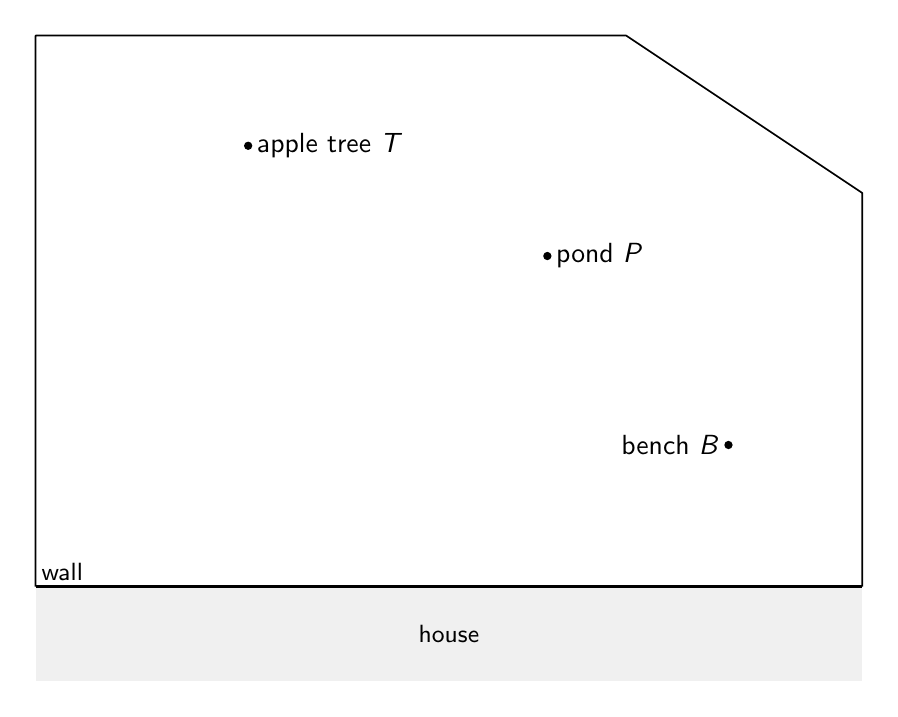
\begin{tikzpicture}[baseline=(current bounding box.north)]
  \useasboundingbox (-0.1,-1.3) rectangle (10.6,7.1);
  % The house, below the wall.
  \fill[black!6] (0,-1.2) rectangle (10.5,0);
  \node[note] at (5.25,-0.6) {house};
  % The fence round the garden, and the wall of the house.
  \draw[line width=0.6pt, line join=round]
    (0,0) -- (0,7) -- (7.5,7) -- (10.5,5) -- (10.5,0);
  \draw[line width=1.2pt] (0,0) -- (10.5,0);
  \node[note, above right] at (0,0) {wall};
  \place{(6.5,4.2)}{right}{pond $P$}
  \place{(2.7,5.6)}{right}{apple tree $T$}
  \place{(8.8,1.8)}{left}{bench $B$}
\end{tikzpicture}
\end{minipage}

\vfill

% Q18: the villages lie on a circle of radius 4 cm, at 200, 320 and
% 85 degrees from its centre, and the mast M is at the centre.
% (d) the third perpendicular bisector passes through M as well.
% (e) M is on the perpendicular bisector of AB, so MA = MB, and on the
% perpendicular bisector of BC, so MB = MC. So MA = MC, and M is
% equidistant from A and C: it is on the perpendicular bisector of AC.
% (f) 4 cm on the map, so 4 x 2 = 8 km.
\noindent
\begin{minipage}[t]{0.47\linewidth}\raggedright
\q Three villages, $A$, $B$ and $C$, are going to share a new phone
mast. The mast must be the same distance from all three villages. The
scale of the map is 1\,cm to 2\,km.
\begin{enumerate}
  \item Construct the locus of the points that are equidistant from
    $A$ and $B$.
  \item Construct the locus of the points that are equidistant from
    $B$ and $C$.
  \item Mark the point $M$ where the mast must be built.
  \item Construct the locus of the points that are equidistant from
    $A$ and $C$. What do you notice?
    \wline
  \item Explain why this happens.
    \wline
    \wline
  \item How far is the mast from each village in real life?
    \answer{1.6cm}{km}
\end{enumerate}
\end{minipage}\hfill
\begin{minipage}[t]{0.5\linewidth}\raggedright
\centering
\begin{tikzpicture}[baseline=(current bounding box.north)]
  \useasboundingbox (-4.5,-4.6) rectangle (4.5,5.4);
  \pt{(200:4)}{left}{A}
  \pt{(320:4)}{right}{B}
  \pt{(85:4)}{above}{C}
\end{tikzpicture}
\end{minipage}

\vfill
\newpage

% ================================================================
% PAGE 8: a treasure map, ending with clues of the pupils' own
% ================================================================

% Q19: (a) the perpendicular bisector of OW crosses the circle of
% radius 4 cm around S at two points, (6.2, 3.9) and (11.1, 4.4)
% measured in cm from the bottom left-hand corner of the map.
% (b) any locus that one position follows and the other does not:
% for example "the treasure is less than 50 m from the oak tree O"
% picks the left-hand point, which is 47 m from O (the right-hand
% point is 93 m from O).
% (c) for example, the distances from X to O, to W and to S: two
% circles meet at two points, and the third circle picks out X. (The
% circles around O and W meet at X and at a second point off the
% left-hand edge of the map, so two clues are enough if pupils say
% that the treasure is on the map.)
\q A treasure map has these two clues. The scale of the map is 1\,cm
to 10\,m.
\begin{itemize}
  \item[] \textbf{Clue 1:} The treasure is the same distance from the
    oak tree $O$ as it is from the well $W$.
  \item[] \textbf{Clue 2:} The treasure is 40\,m from the standing
    stone $S$.
\end{itemize}

\begin{diagram}
\begin{tikzpicture}
  \useasboundingbox (-0.1,-0.1) rectangle (13.1,7.6);
  \draw[line width=0.6pt, rounded corners=4pt] (0,0) rectangle (13,7.5);
  \place{(2.5,1)}{right}{oak tree $O$}
  \place{(2,6)}{right}{well $W$}
  \place{(9,1)}{right}{standing stone $S$}
  \pt{(8.5,6.3)}{right}{X}
\end{tikzpicture}
\end{diagram}

\vspace{6pt}
\begin{enumerate}
  \item Use both clues to mark the possible positions of the treasure.
  \item Write a third clue that tells you which of the positions is the
    treasure. Your clue must describe a locus.
    \wline
    \wline
  \item More treasure is buried at the point $X$. Write some clues that
    lead to $X$ and to no other point on the map. Use as few clues as
    you can, and check your clues by constructing their loci on the
    map.
    \wline
    \wline
    \wline
    \wline
\end{enumerate}

\vfill

\end{document}
